\documentclass[11pt,letterpaper]{article}
\usepackage[utf8]{inputenc}
\usepackage[margin=1in]{geometry}
\usepackage{amsmath}
\usepackage{amsfonts}
\usepackage{amssymb}
\usepackage{amsthm}
\usepackage{verbatim}
\usepackage{graphicx}
\usepackage{sidecap}
% No paragraph tabs
\setlength{\parindent}{0pt}

% Define commands that will be widely used.
\newcommand{\br}{\ \\}
\newcommand{\tab}{\hspace*{2em}}

\title{Optical Pumping and the Nuclear Spin of Rubidium}
\author{Rachel Domagalski\\
Partner: Matthew Turner}
\date{October 21, 2013}

\begin{document}
\maketitle

\begin{abstract}
    Quantum mechanics predicts several energy level splittings due to the inner
    structure of the atom, as well as energy level splittings due to external
    manipulations, like an external magnetic field. Combinations of these energy
    level splittings can be used to pump electrons into higher energy level
    states, which is the essence of the optical pumping process. This experiment
    uses optical pumping to measure the nuclear spin of a couple of Rubidium
    isotopes and then uses those spins to estimate the strength of the Earth's
    magnetic field at UC Berkeley. The values of the nuclear spins of $^{85}Rb$
    and $^{87}Rb$ were measured to be 5/2 and 3/2 respectively and the strength
    of the Earth's magnetic field was measured to be $0.333 \pm 0.002$ Gauss.
\end{abstract}

\section{Introduction}

\subsection{Theory}

\begin{figure}
    \centering
    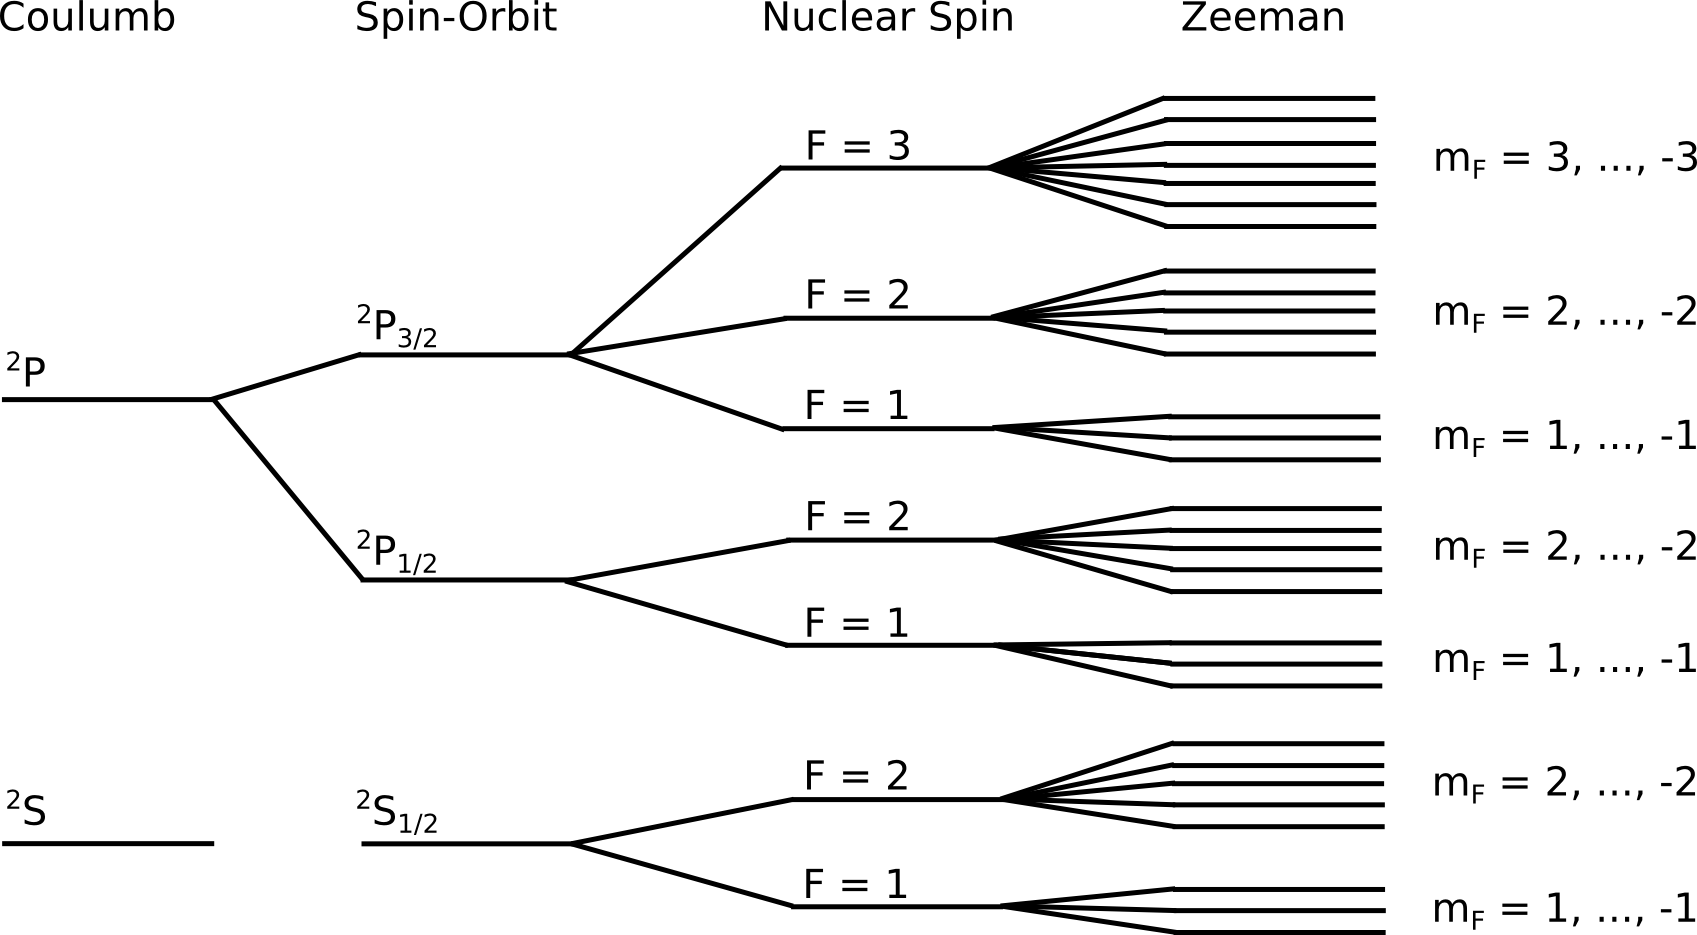
\includegraphics[width=\textwidth]{figures/splittings.png}
    \caption{Diagram of the energy level splittings studied in the optical
    pumping experiment. Energy levels are not to scale.}
    \label{optenergylvl}
\end{figure}

\begin{figure}
    \centering
    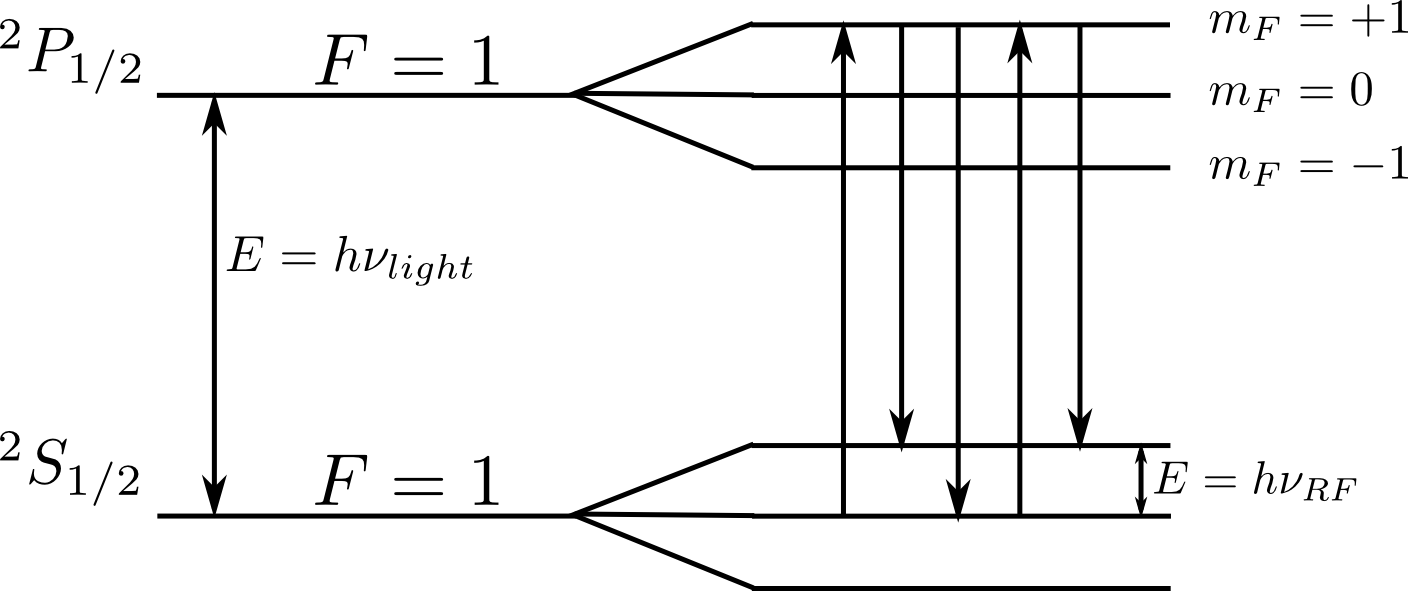
\includegraphics[width=\textwidth]{figures/opticalpumping.png}
    \caption{Simplified diagram of the process of optical pumping using only one
        large energy jump. In the actual experiment, transitions from all of the
        other energy levels will occur.}
    \label{optpump}
\end{figure}

In quantum mechanics, the study of energy level splittings is of high
importance. The framework of quantum mechanics is very applicable to the study
of atomic structure. Several natural energy level splittings related to atomic
structure (see Figure \ref{optenergylvl}) that occur include the Coulomb
interaction between the electron and nuclear charge, the spin-orbit interaction,
and an interaction from the nuclear spin. These splittings are included in the
Hamiltonian of the system, but they cannot be manipulated by an experimenter.
While splittings related to the structure cannot be touched, a further splitting
of the energy levels can be induced by applying an external magnetic field to
the electrons, and this splitting as a quantum number $m_F$. Splitting from an
external magnetic field is called Zeeman splitting.\\

A relationship between the Zeeman splitting frequency and an external magnetic
field is given by the Breit-Rabi formula \cite{LabManual},
\begin{equation}
    \frac{\nu}{B_{ext}} = \left(\frac{2.799}{2I+1}\right)\ MHz/gauss
    \label{breitrabi}
\end{equation}
where $I$ is the nuclear spin. When the direction used for measuring spin is
aligned with the Earth's magnetic field and if no external field is applied,
then the strength of the Earth's magnetic field can determined from measuring
the splitting frequency, assuming that the nuclear spin is known. In fact, the
Earth's magnetic field is measured in this experiment.\\

The optical pumping experiment is done with the Rubidium element in gas form
and a rough visualization of the optical pumping process can be seen in Figure
\ref{optpump}. The general principle behind optical pumping is to raise
electrons into higher $m_F$ states. This is done by shining circularly polarized
light onto a bulb of Rubidium gas. Because of the polarization of the light, the
electron can only make $\Delta m_F = +1$ jumps during when it absorbs a photon.
After a while, the electron emits a photon and makes a jump where $\Delta m_F =
0, \pm 1$. Once all of the electrons are pumped up, the Rubidium gas cannot
absorb any more light. In order for the pumping process to be repeated, a radio
frequency (RF) field must be applied to cause the electrons to transition back
down to a lower $m_F$ state.\\

Figure \ref{optpump} illustrates an example to demonstrate why the optical
pumping technique forces electrons into higher $m_F$ states. In the figure,
electrons are able to move from subsets of two $F = 1$ states involved in the
experiment. Suppose that an electron is in the $m_F = 0$ state for the
$^2S_{1/2}$ level. When it absorbs a photon, it will move up to the $m_F = 1$
state in the $^2P_{1/2}$ level. When losing a photon, the electron will either
move to the $m_F = 1$ state or the $m_F = 0$ state, with roughly 50\%
probability for going into either state. If the electron goes to the $m_F = 1$
state, it is done, as the $P$ level doesn't have an $m_F = 2$ state. When $m_F =
0$, the process just repeats from the beginning. Clearly, this process leads to
electrons going to the higher $m_F$ states.

\subsection{Experimental Setup}

\begin{figure}
    \centering
    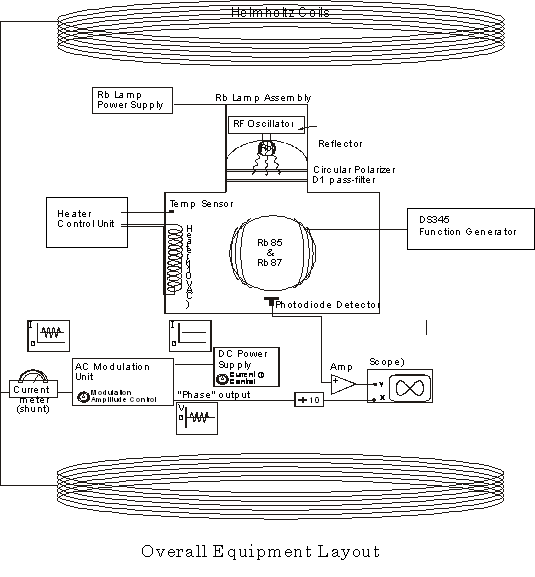
\includegraphics[width=0.9\textwidth]{figures/OPTimage001.png}
    \caption{Block diagram of the optical pumping experiment \cite{LabManual}.}
    \label{optbd}
\end{figure}

The experimental setup for the optical pumping lab is pretty straightforward,
and can be seen in Figure \ref{optbd} \cite{LabManual}. Rubidium gas contained
in a bulb is placed in a box, which contains circuitry to measure the
temperature, shine circularly polarized light at the Rubidium (see the Theory
section for description of the optical pumping process), oscillate a radio
frequency, and measure emitted light from the Rubidium. The Rubidium gas
contains both $^{85}Rb$ and $^{87}Rb$, as will be seen in the Experimental
Methods section.\\

To induce Zeeman splitting, an external magnetic field is produced from
Helmholtz coils as well as the Earth's magnetic field. The Earth's magnetic
field determines the direction that spin is measured on, and thus the field from
the Helmholtz coils must point in the same direction of the Earth's field. The
field inside of a Helmholtz coil is relatively uniform, which makes it a good
choice for this experiment. The total magnetic field applied to the Rubidium is
\cite{LabManual}
\begin{equation}
    \vec{B}_{ext} = \vec{B}_{E} \pm 0.9 \times 10^{-6} \left(\frac{tesla \cdot
    meter}{ampere} \right) \frac{Ni}{a} \hat{n}
    \label{totalbext}
\end{equation}
where $\vec{B}_E$ is the Earth's magnetic field, $N$ is the number of turns in
the coil, $i$ is the current in the coil, $a$ is the radius of the coil, and
$\hat{n}$ is the direction normal to the planes made from the coil. The $\pm$
depends on the polarity of the current running through the coil.\\

The other main components of the experiment are the AC modulation unit and the
heater control unit. The AC modulator takes in a DC current source and sends it
to the coils. This is necessary because some parts of the experiment require a
modulated field from the Helmholtz coil, which will be described in the
Experimental Method section. The temperature control is important because the
optical signal strength of the Rubidium depends on how hot the gas is. The ideal
temperature to operate this experiment can be seen in Figure \ref{tempcalib}
\cite{LabManua}. It should be noted that the heater unit should not be turned on
while making measurements. This is because it has its own coil, which produces a
magnetic field when turned on and disturbs the experiment. Fortunately, the
temperature of the bulb drops slowly enough so that many measurements can be
made before needing to reheat the bulb.

\begin{figure}
    \centering
    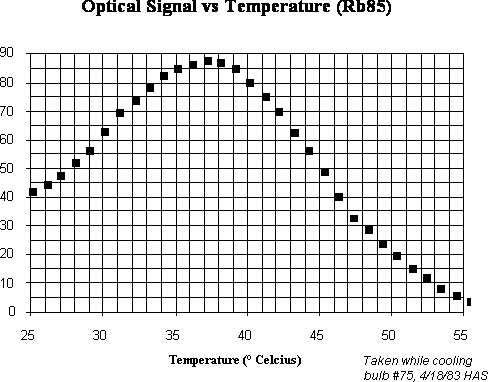
\includegraphics[width=0.6\textwidth]{figures/OPTimage006.png}
    \caption{The optical signal strength for $^{85}Rb$ is relatively flat
    between $35^\circ C$ and $40^\circ C$ \cite{LabManual}.}
    \label{tempcalib}
\end{figure}

\section{Experimental Method}

\subsection{Opacity of Rubidium}

One method of measuring the resonance frequency for a given current is to set
the current in the Helmholtz coil to some constant value and to ramp the RF from
the function generator controlling it \cite{LabManual}. The way to do this is
choose a range of frequencies as the span of the function generator and set the
carrier frequency as about half of the span. In order for this to work, the span
must be larger than the resonance frequencies of the isotopes, else the isotopes
will not be seen. The physics of what is going on is that the function generator
is attempting to match the splitting frequency for some fixed magnetic field, as
governed by the Breit-Rabi formula \eqref{breitrabi}. The actual resonance
frequency is acquired by sending the modulation output of the function generator
to the first channel on the oscilloscope, and the output of the photodetector
through and amplifier and to the second channel on the scope. When the scope is
set to X-Y mode, the resonance frequency for a specific isotope by finding the
peak signal for that isotope. An example of this for a Rubidium bulb containing
only $^{87}Rb$ can be seen in Figure \ref{rb87opacity}. Since the resonance
frequency of the Rubidium really only depends on the strength of the magnetic
field, the measured resonance is pretty much invariant on the span and carrier
frequency from the function generator, and that was observed in the experiment.

% Plot modulating the RF and seeing the signal
\begin{figure}
    \centering
    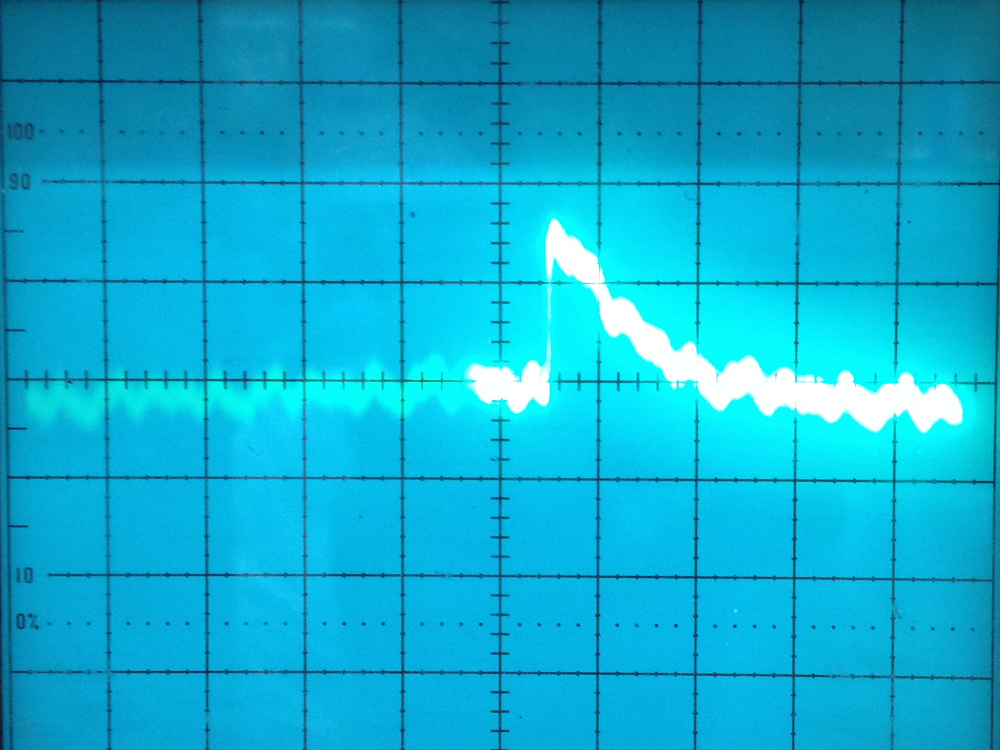
\includegraphics[width=0.6\textwidth]{figures/IMG_1241.JPG}
    \caption{Opacity measurement featuring the bulb that only contained
        $^{87}Rb$. Since the X axis is the modulation output, it can be easily
        translated to a frequency measurement.}
    \label{rb87opacity}
\end{figure}

\subsection{Increasing precision of the resonance frequency}

The above method for determining the resonance frequency is very imprecise and
should not be used, as more precise methods are available. The method used to
determine the resonance frequency goes as follows. First, modulation is turned
off for the RF and on for the external magnetic field. The modulation frequency
of the magnetic field is set to 60 Hz and the modulation amplitude is set to
roughly 30 mA. The phase output and photodetector signals can now be displayed
in X-Y mode on the oscilloscope and their shape forms a Lissajous figure, which
can be used to determine the resonance frequency. The resonance frequency for a
magnetic field strength is the frequency that makes the Lissajous figure the
most symmetric about the Y axis. An example of this can be seen in Figure
\ref{lissajous}.\\

\begin{figure}
    \centering
    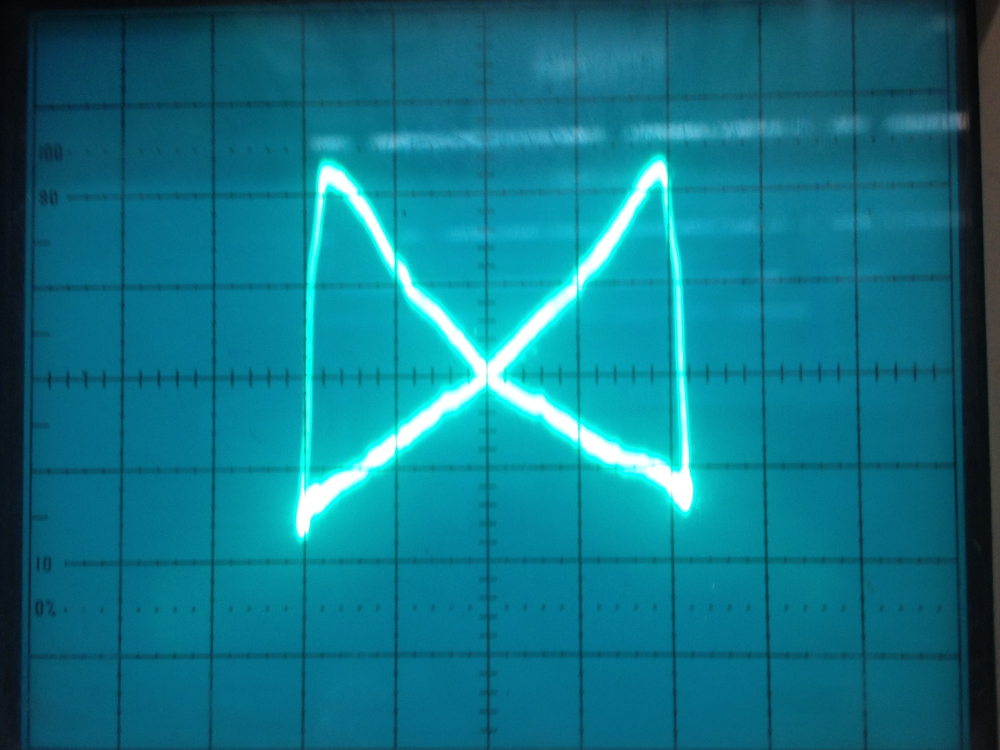
\includegraphics[width=0.6\textwidth]{figures/IMG_1242.JPG}
    \caption{The resonance frequency can be found by making a symmetric
    Lissajous figure in X-Y mode of the scope. The X axis is the phase output of
    the AC modulation unit, whereas the Y axis is the amplified output of the
    photodetector.}
    \label{lissajous}
\end{figure}

The reason that the above method works in finding the resonance frequency is as
follows and a visualization of it can be seen in Figure \ref{resdemo}. Suppose
that the frequency from the function generator is set to some value near the
resonance frequency for the magnetic field given by the input current. Because
of the modulation of the field, the strength of the field will oscillate to the
strength for which the applied RF is at resonance. If that strength is far from
the magnetic field strength of the center of modulation, then the time
differences between when the field reaches the strength of the field for
resonance alternate between being a longer period and a shorter period, which
will result in an asymmetry on the Lissajous figure. As can be seen from Figure
\ref{resdemo}, when the field that will cause RF to be the resonance frequency
is closer to the center field strength of the modulation, the periods between
when the field is at that resonant strength become more consistent and even,
which results in a symmetric Lissajous figure. By setting the RF to a value
where the Lissajous figure becomes symmetric, the resonance frequency for the
magnetic field strength can be found. Of course, there will be some range in the
frequencies that give a symmetric Lissajous pattern, and that is a systematic
error in the measurement process that must be noted and accounted for. Ideally,
that systematic error should be small and the resonance frequency for a given
magnetic field strength can be easily found.

\begin{figure}
    \centering
    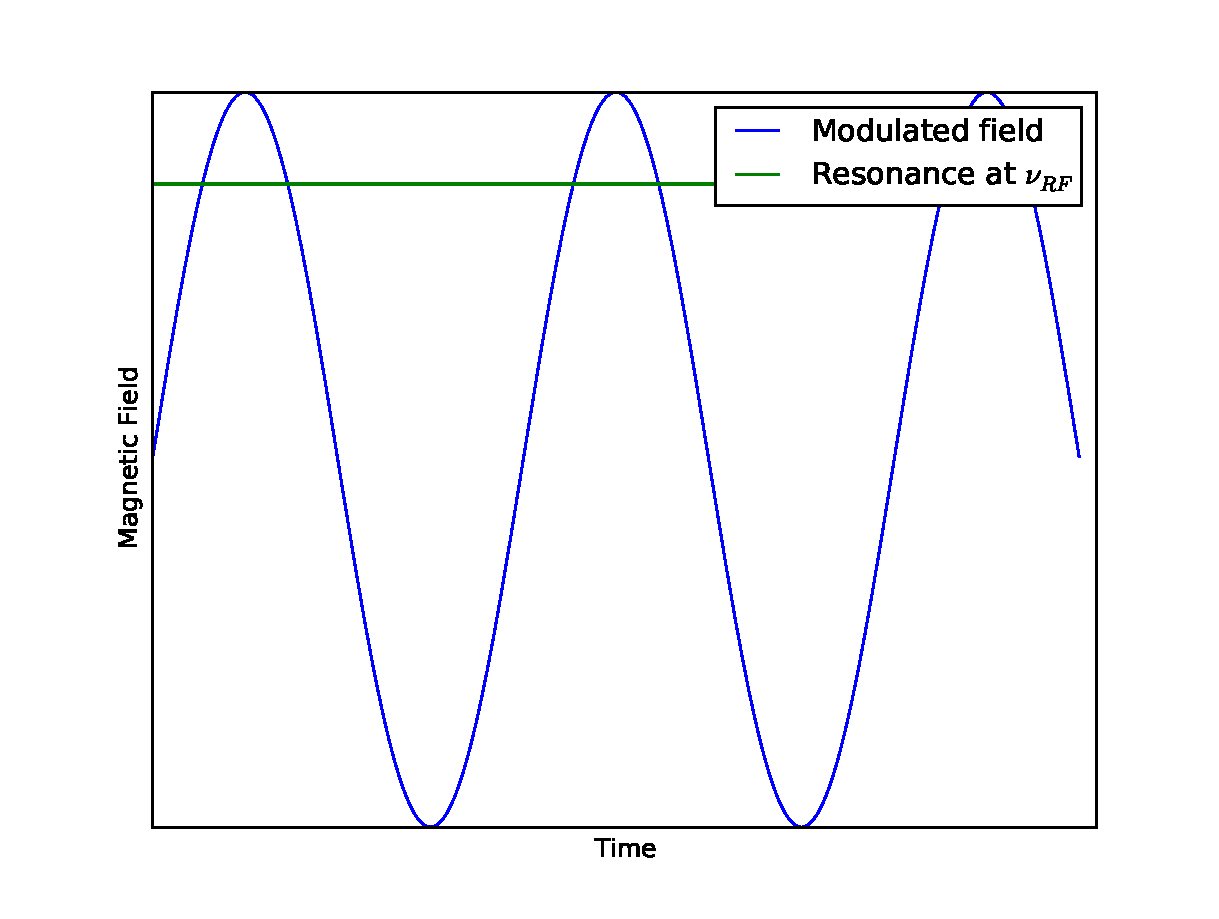
\includegraphics[width=0.6\textwidth]{figures/resonance_demo.pdf}
    \caption{Demonstration for why the symmetry of the Lissajous figure is a
    good way to determine the resonance frequency.}
    \label{resdemo}
\end{figure}

\section{Analysis}

\subsection{Nuclear spin}

Equations \eqref{breitrabi} and \eqref{totalbext} can easily be manipulated to
give the following relationship between current and frequency:
\begin{equation}
    \nu = \left(\frac{2.799}{2I+1}\frac{0.9\times 10^{-2} N}{a} \right) i
        + \left(\frac{2.799}{2I+1}\right) B_E
    \label{brexpanded}
\end{equation}
This formula is useful because it provides a method of calculating the nuclear
spin from a linear fit of the data. Using a fit of $y = mx + b$, it can shown
that $I$ can be calculated as
\begin{equation}
    I = \frac{1}{2}\left(\frac{2.5191 \times 10^{-2} N}{ma} - 1\right)
    \label{nucspin}
\end{equation}
where $m$ is the slope of the linear fit, $a$ is the radius of the Helmholtz
coil, and $N$ is the number of turns of the coil. Of course, $I$ must be a half
integer and there is really no guarantee that \eqref{nucspin} will give out such
a number. However, the value for $I$ computed from \eqref{nucspin} has an error
associated with it, and the nuclear spin should be the closest half integer to
the value of $I$ computed from \eqref{nucspin} within some error associated with
the measurement.

\subsection{Earth's magnetic field}

Equation \eqref{brexpanded} might suggest that the Earth's magnetic field can be
calculated using the intercept of a linear fit. While this is true, there is a
better way to do calculate it. Suppose that for every time the Helmholtz coil
has a positive current, a measurement is made where the polarity on the current
is flipped. This will cause a slightly different resonance frequency for the
Rubidium. These two resonance frequency pairs have the following values
\cite{LabManual}:
\begin{equation}
    \nu^+ = \left(\frac{2.799}{2I+1}\right) \left|B_H + B_E\right|
\end{equation}
\begin{equation}
    \nu^- = \left(\frac{2.799}{2I+1}\right) \left|-B_H + B_E\right|
\end{equation}
In the above equations, $\nu^-$ can be thought of as a negative frequency, but
in reality, all frequency measurements are positive. Clearly, these two
frequencies can be added together to get the Earth's magnetic field, which is
given as
\begin{equation}
    B_E = \frac{1}{2}\left(\frac{\nu^+-\nu^-}{2.799}\right) (2I+1)
\end{equation}
and it should be stressed that the value used for $\nu^-$ is the positive
measurement. Since this can be done for every $\nu^\pm$ pair, the Earth's
magnetic field can be computed by taking the average of all pairs, which makes
calculating the uncertainty of the Earth's field incredibly straightforward.

\subsection{Error analysis}

Since the value of the nuclear spin is exactly a half integer, a full error
analysis for the spin is not needed. However, the measurements of the resonance
frequency do have errors and these must be accounted for. There are two ways to
get the error of the frequency measurements. The first way is to measure the
range over which the Lissajous figure looks symmetric. In the actual experiment,
this error was approximately 1 kHz for currents less than 1.6 A and about 5 kHz
for currents greater than 1.6 A.\\

The second way to calculate the error of the resonance frequency is to determine
what error would be needed for a linear fit to have $\chi^2 / ndf = 1$. This
method can be quickly derived from the definition of $\chi^2$, which is
\cite{LyonsError}
\begin{equation}
    \chi^2 = \sum_{i=1}^{n}\left(\frac{y_i - m x_i - b}{\sigma_i} \right)^2
\end{equation}
If it assumed that $\sigma_i$ is the same for every $y_i$, and that the value of
$\chi^2$ is equal to $ndf$, one can solve for $\sigma$. This yields
\begin{equation}
    \sigma_{RF} = \sqrt{\frac{1}{n-2}\sum_{i=1}^n \left(y_i-mx_i-b\right)^2}
\end{equation}
where $n$ is the number of data points used in the least squares fit.\\

The uncertainty of the Earth's magnetic field is very straightforward to
calculate, as the field is computed by taking a mean. The error of the field
from individual measurements only really depends on the combined error of
$\nu^+$ and $\nu^-$. Since this error is the same for all individual field
measurements, there is no difference between taking a weighted mean or an
unweighted mean, and the error on the mean strength of the earth's magnetic
field is the desired uncertainty.

\section{Results}

\begin{figure}
    \centering
    \begin{minipage}[t]{0.49\textwidth}
        \centering
        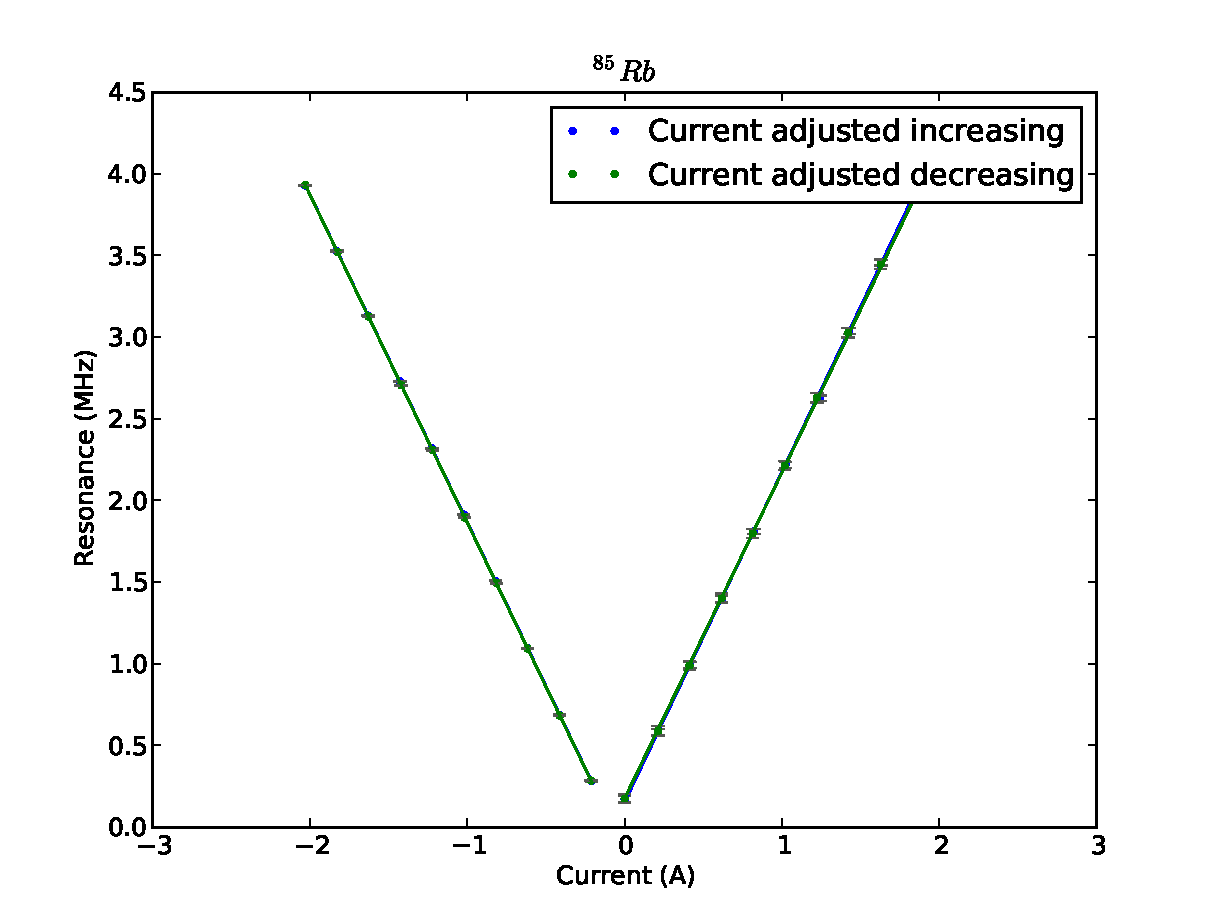
\includegraphics[width=\textwidth]{figures/rubidium85.pdf}
    \end{minipage}
    \begin{minipage}[t]{0.49\textwidth}
        \centering
        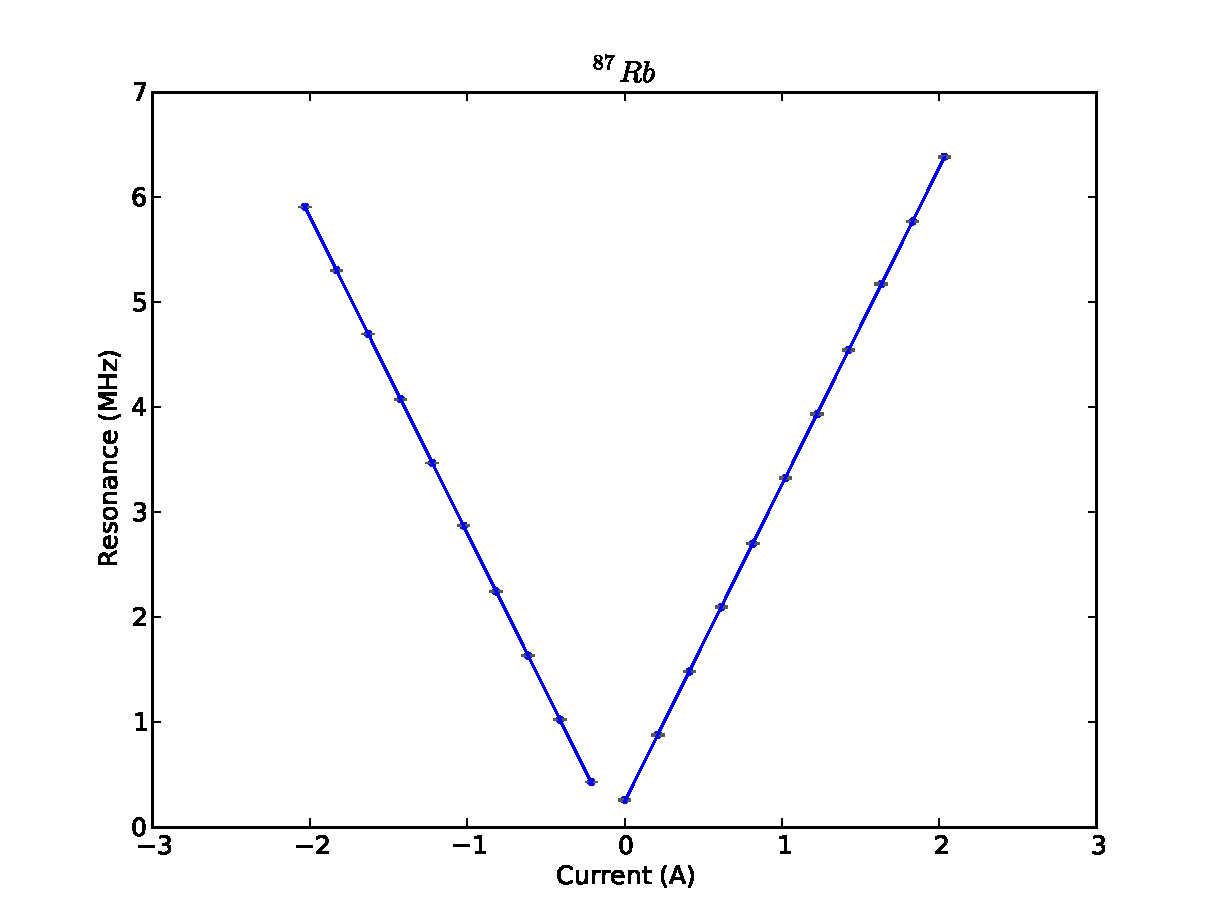
\includegraphics[width=\textwidth]{figures/rubidium87.pdf}
    \end{minipage}
    \caption{Nuclear spin can be calculated with a linear fit of the data. Error
        bars are printed on the plot, but the errors are small. (left) The plot
        for $^{85}Rb$ shows that hysteresis effects are relatively minimal and
        can be neglected. (right) Plot for $^{87}Rb$.}
    \label{currentfrequency}
\end{figure}

The nuclear spins of both Rubidium isotopes was calculated by fitting the slopes
of the lines fit to the Breit-Rabi formula, which can be seen in Figure
\ref{currentfrequency}. It should be noted that there are two curves in the left
figure. That was to test for hysteresis effects in the AC modulation unit. If
hysteresis was large, then there would be some notable separation between the
blue and green lines, and a correction would have to have been made for it.
However, hysteresis was small, so no correction needed to be made and this
effect therefore was not measured with measuring the spin of $^{87}Rb$. The
uncertainties on RF were 0.018 Hz for positive current on $^{85}Rb$, 0.003 Hz
for negative current on $^{85}Rb$, 0.008 Hz for positive current on $^{87}Rb$,
and 0.003 Hz for negative current on $^{87}Rb$. The spins measured from the
linear fits were 2.4 and 1.4 for $^{85}Rb$ and $^{87}Rb$ respectively, which
implies that the spins of these isotopes are 5/2 and 3/2, which are the accepted
values for these isotopes. The value of the Earth's magnetic field was
calculated to be $0.333 \pm 0.002$ Gauss, which is a reasonable measurement.
Details of the analysis code used to compute these results can be found at
https://bitbucket.org/domagalski/physics111-advanced-lab/ \cite{Bitbucket}.

\bibliographystyle{unsrt}
\bibliography{ReferenceList}{}

\end{document}
